% 编译使用xelatex编译一次

\documentclass[12pt, a4paper, oneside]{ctexart}
\usepackage{subcaption,listings,amsmath, amsthm, amssymb, bm, booktabs, color, framed,float, graphicx, hyperref, mathrsfs,minipage-marginpar}

\title{\textbf{数据库系统作业五}}
\author{2021113140符世博}
\date{}
\linespread{1.5}
\definecolor{shadecolor}{RGB}{241, 241, 255}
\newcounter{problemname}
\newenvironment{problem}{\begin{shaded}\stepcounter{problemname}\par\noindent\textbf{题目\arabic{problemname}. }}{\end{shaded}\par}
\newenvironment{solution}{\par\noindent\textbf{解答. }}{\par}
\newenvironment{note}{\par\noindent\textbf{题目\arabic{problemname}的注记. }}{\par}

\begin{document}
\maketitle

% 1
\begin{problem}
    考虑在公共属性$a$上的连接关系$R(a,b)$和$s(a,c,d)$,假设表上没有可用的索引来加速连接算法。

    缓冲区中有$B=75$页

    表$R$包含$M=2400$个页面,每个页面包含$80$个元组

    表$S$包含$N=1200$个页面,每个页面包含$100$个元组

    请回答一下关于计算连接的I/O开销的问题。你可以假设最简单的开销模型,即每次只读写一个页面。你还可以假设你需要一个缓冲块来保存演变中的输出块,
    以及一个输入块来保存内部关系的当前输入块。你可以忽略最终结果的成本。

    A.\quad 以$R$为外部关系,$S$为内部关系的块嵌套循环连接

    B.\quad 以$S$为外部关系,$R$为内部关系的块嵌套循环连接
\end{problem}

\begin{solution}
    A.\quad 共产生$2400+\frac{1200\times 2400}{75-2}=40653$次IO操作

    B.\quad 共产生$1200+\frac{2400\times 1200}{75-2}=39453$次IO操作
\end{solution}

% 2
\begin{problem}
    设关系$R(X,Y)$和$S(Y,Z)$,$R$共有$1000$个元组,$S$共有$1500$个元组,每个块种可容纳$20$个$R$元组或$50$个$S$元组。$S$中$Y$不同值的个数为$20$。

    (1)\quad 若在$S.Y$上建有聚簇索引,估计$R$和$S$基于索引连接的$IO$查询代价。

    (2)\quad 若在$S.Y$上建有非聚簇索引,估计$R$和$S$基于索引连接的$IO$查询代价。
\end{problem}

\begin{solution}
    (1)\quad IO查询代价为$B(R)+T(R)\lceil\frac{B(S)}{V(S,Y)}\rceil=50+1000\times\lceil\frac{30}{20}\rceil=2050$

    (2)\quad IO查询代价为$B(R)+\frac{T(R)T(S)}{V(S,Y)}=50+\frac{1000\times 1500}{20}=75050$
\end{solution}

% 3
\begin{problem}
    已知两个关系$R(A,B)$和$S(B,C)$,其主键分别为$R.A$和$S.B$。$R$有$40000$个元组,$S$有$60000$个元组,一块中可以容纳$20$个$R$元组或
    $30$个$S$元组。设$2$个关系均采用聚簇存储,且每个关系中的元组均已按照其主键值递增排序。现在要执行自然连接操作$R\Join S$。设缓冲区中可用内存页数为$M=41$。回答下列问题:

    (1)\quad 采用嵌套循环连接算法执行$R\Join S$分别需要进行多少次$I/O$?给出具体分析过程。

    (2)\quad 采用归并连接算法执行$R\Join S$分别需要进行多少次$I/O$?给出具体分析过程。

    (3)\quad 设$R.B$是关系$R$的外键,参照$S.B$。如果$R\Join S$的结果中元组的平均大小是$R$中元组平均大小的$1.2$倍,$R\Join S$的结果中元组的平均大小是$S$中元组平均大小的$2$倍,那么在外存中存储$R\Join S$的结果需要占用多少个块(页)?给出具体分析过程。
\end{problem}

\begin{solution}
    (1)\quad 采用基于块的循环嵌套连接,由于B(R)<B(S),所以选择R作为外关系。那么IO次数$=B(R)+\frac{B(R)B(S)}{M-1}=2000+\frac{2000\times 2000}{41-1}=102000$

    (2)\quad 由于关系R在属性B上并不是有序的,所以需要先对它划分归并段。由于关系S在属性B上时有序的所以在归并时可认为其只有一个归并段。因此,对于关系R,创建的归并段至多有40个。经过一次排序后,对于关系R可以创建$\lceil\frac{B(R)}{M}\rceil=\lceil\frac{2000}{41}\rceil=49$个归并段。
所以,还需要进行一次排序,经过两次排序后,关系R得到了两个归并段。这时已经产生了$4B(R)$次IO操作。在归并阶段时,又会产生$B(R)+B(S)$次IO操作,所以一共有$5B(R)+B(S)=5\times 2000+2000=12000$次IO操作。

    (3)\quad 
\end{solution}

% 4
\begin{problem}
    设教学管理数据库有如下3个关系模式:

    $S(S\#,SNAME,AGE,SEX)$

    $C(C\#,CNAME,TEACHER)$

    $SC(S\#,C\#,GRADE)$

    其中$S$为学生信息表、$SC$为选课表、$C$为课程信息表;$S\#$、$C\#$分别为$S$、$C$
    表的主码,$(S\#,C\#)$是$SC$表的主码,也分别是参照$S$、$C$表的外码
    用户有一查询语句:

    Select\quad SNAME
    
    From\quad S,SC,C

    Where\quad SC.S\#=S.S\#\quad and\quad SC.C\#=C.C\#\quad and \quad CNAME="数据库";

    检索选学“数据库”课程的学生的姓名。
    
    (1)写出以上 $SQL$ 语句所对应的关系代数表达式。

    (2)画出上述关系代数表达式所对应的查询计划树。 使用启发式查询优化算法,
    对以上查询计划树进行优化, 并画出优化后的查询计划树。

    (3)设 $SC$ 表有 $10000$ 条元组, $C$ 表有 $50$ 条元组, $S$ 表中有 $1000$ 条元组, $SC$
    中满足选修数据库课程的元组数为 $150$, 计算优化前与优化后的查询计划中
    每一步所产生的中间结果大小。
\end{problem}

\begin{solution}
    (1)\quad $\Pi_{S.SNAME}(\sigma_{SC.S\#=S.S\#\quad and\quad SC.C\#=C.C\#\quad and\quad C.CNAME='\text{数据库}'}(S\times (C\times SC)))$

    (2)

    \begin{figure}[H]
        \centering
        \begin{minipage}[c]{0.45\textwidth}
            \centering
            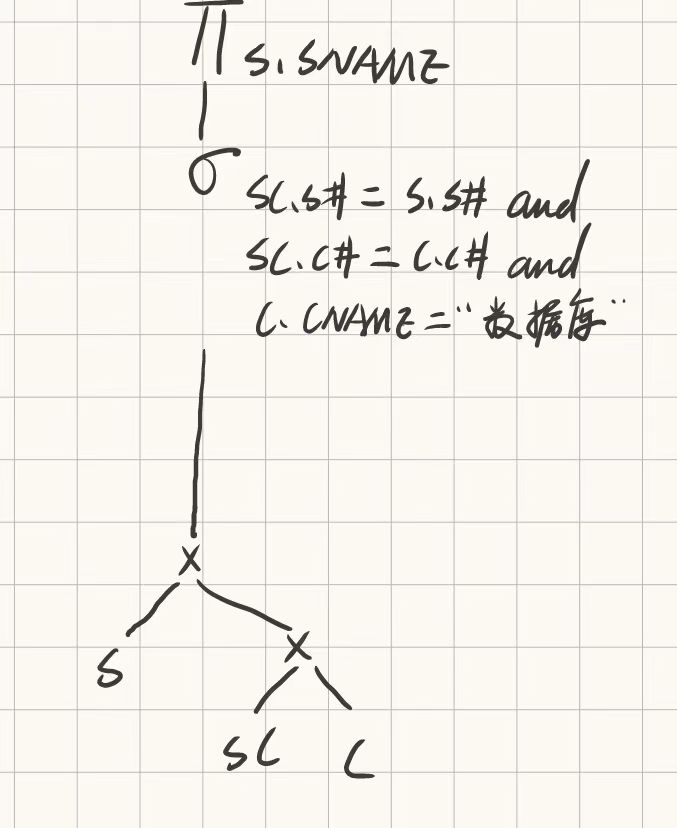
\includegraphics[width=0.95\textwidth]{figures/1.jpg}
            \subcaption{查询计划树}
        \end{minipage}
        \begin{minipage}[c]{0.45\textwidth}
            \centering
            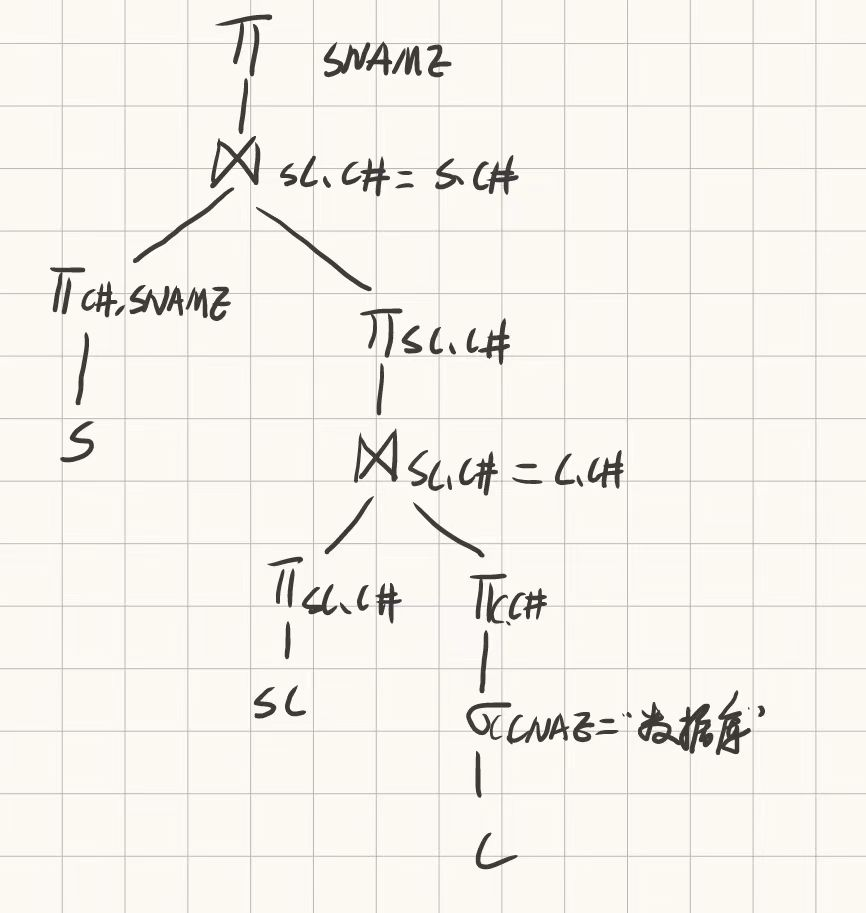
\includegraphics[width=0.95\textwidth]{figures/2.jpg}
            \subcaption{优化后的查询计划树}
        \end{minipage}
    \end{figure}

    (3)
    如下图,图中标注该操作产生的元组个数。

    \begin{figure}[H]
        \centering
        \begin{minipage}[c]{0.45\textwidth}
            \centering
            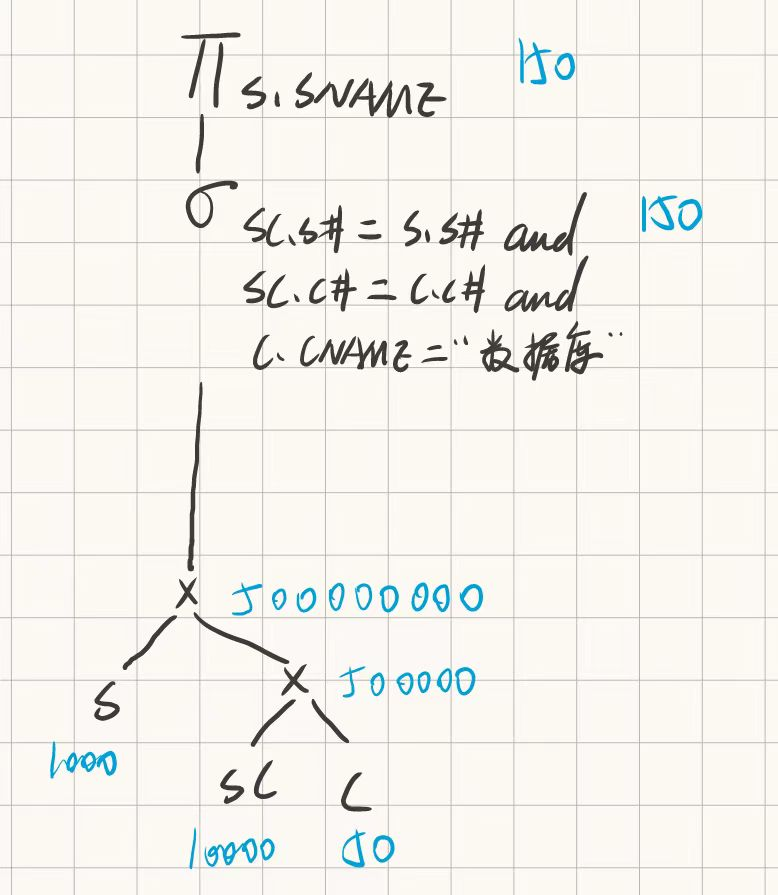
\includegraphics[width=0.95\textwidth]{figures/3.jpg}
            \subcaption{优化前}
        \end{minipage}
        \begin{minipage}[c]{0.45\textwidth}
            \centering
            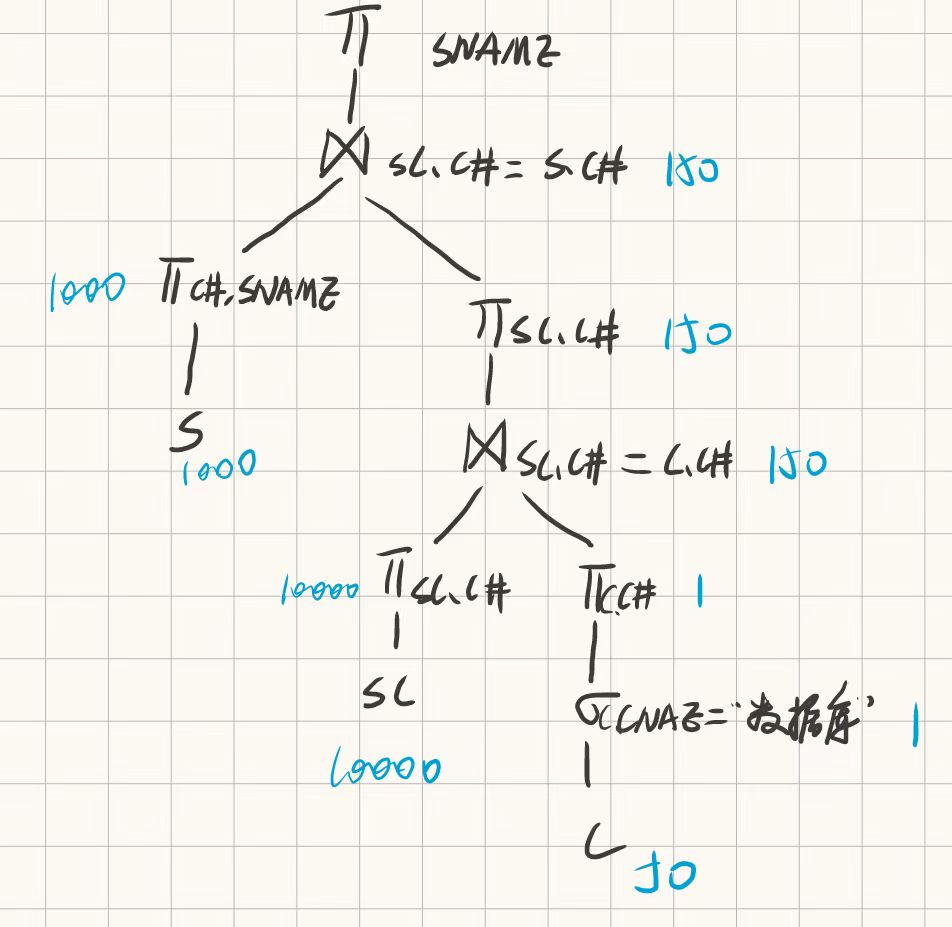
\includegraphics[width=0.95\textwidth]{figures/4.jpg}
            \subcaption{优化后}
        \end{minipage}
    \end{figure}
\end{solution}

% 5
\begin{problem}
    给定以下关系模式

    $Student (sid, sname, major)$

    $Course (cid, cname, credit)$

    $Enrollment (sid, cid, grade)$

    (1) 考虑以下的 $SQL$ 查询语句, 绘制其查询计划树

    SELECT C.name

    FROM Student S, Course C, Enrollment E

    WHERE S.sid = E.sid

    AND C.cid = E.cid

    AND S.major = 'Computer Science'

    AND C.credit >= 90;

    (2) 假设在$Student.major$和$Enrollment.sid$上建有索引, 绘制优化后的查询计划树。
\end{problem}

\begin{solution}
    (1)

    \begin{figure}[H]
        \centering
        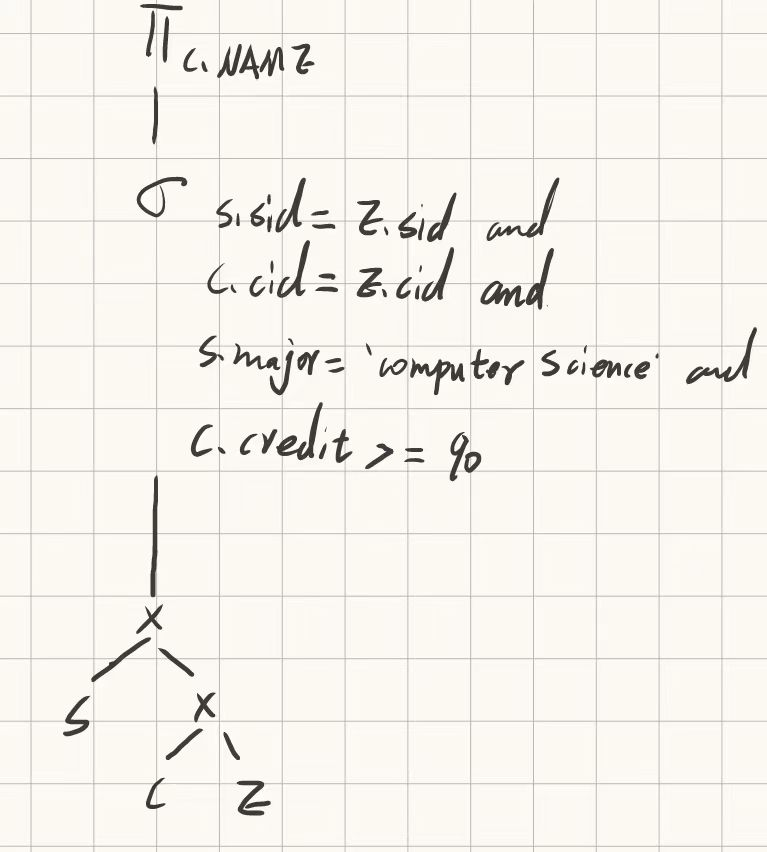
\includegraphics[width=0.95\textwidth]{figures/5.jpg}
    \end{figure}

    (2)

    \begin{figure}[H]
        \centering
        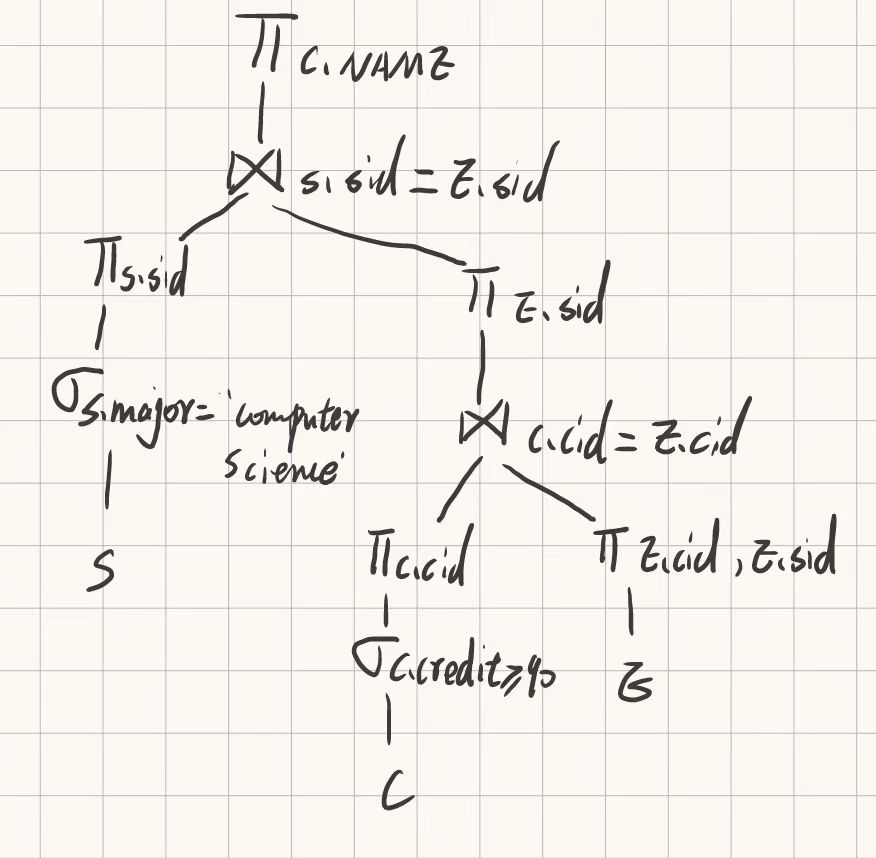
\includegraphics[width=0.95\textwidth]{figures/6.jpg}
    \end{figure}

\end{solution}

% 6
\begin{problem}
    已知一个关系数据库的模式如下:

    关系 $B(\underline{bno}, bname, author)$为图书表, 其中 $bno$ 为书号, $bname$ 为书名, $author$
    为作者;

    关系 $S(\underline{sno}, sname, dept)$为学生表, 其中 $sno$ 为学号, $sname$ 为姓名, $dept$ 为学
    生所在系;

    关系 $L(\underline{sno} , bno, date)$为借书表, 其中 $sno$ 为学号, $bno$ 为书号, $date$ 为借书时
    间。

    回答下列问题:

    (1) 绘制下面的 $SQL$ 查询语句的逻辑查询计划树。

    SELECT author FROM B NATURAL JOIN S NATURAL JOIN L
    
    WHERE date = ‘2023-11-01’ AND dept = ‘Math’;

    (2) 使用启发式查询优化方法对上面的逻辑查询计划树进行优化, 绘制优化后得
    到的逻辑查询计划树, 具体说明你进行这些优化的理由。
\end{problem}

\begin{solution}
    (1)

    \begin{figure}[H]
        \centering
        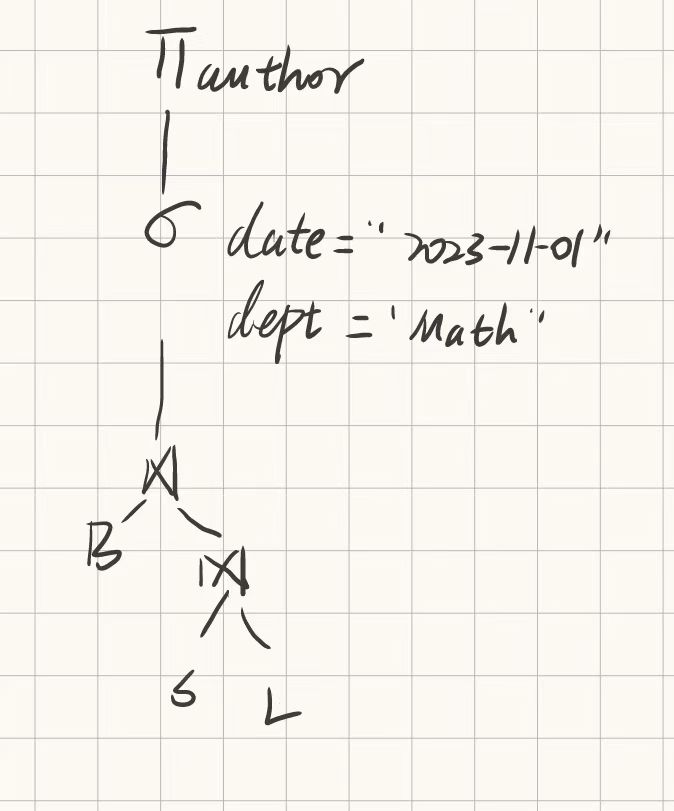
\includegraphics[width=0.95\textwidth]{figures/7.jpg}
    \end{figure}

    (2)

    \begin{figure}[H]
        \centering
        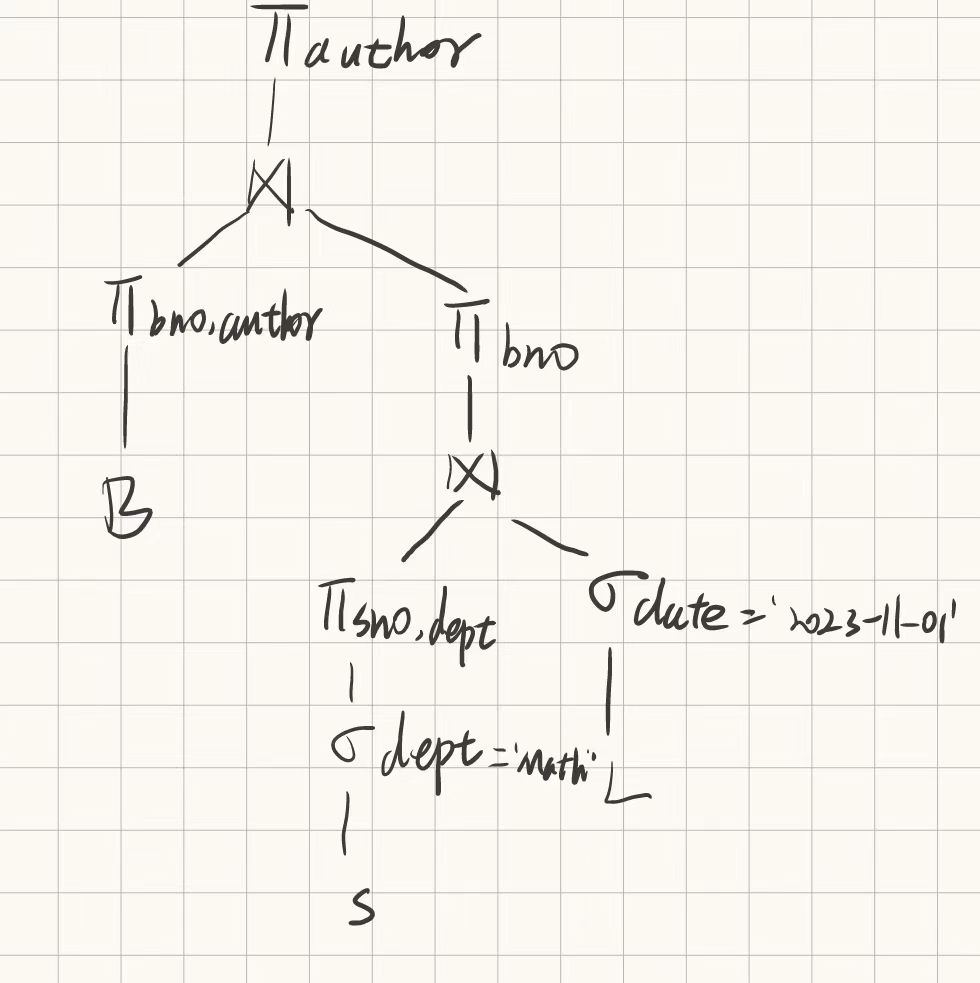
\includegraphics[width=0.95\textwidth]{figures/8.jpg}
    \end{figure}

    将投影和选择尽可能的早执行,同时利用投影操作筛选后续操作中不必要的属性,减少执行过程中的元组个数。
\end{solution}



\end{document}